\documentclass[main.tex]{subfiles}
\begin{document}
\chapter{Multitasking的正确性}\label{chp:proof_multi}
我们首先定义一些概念,它们类似\cite{soltanolkotabi2011geometric}中的提法。

\begin{definition}[投影对偶空间]\label{def:proj_dual_direction}
  令 $N$ 为下面对偶问题的最优解
  \begin{align*}
    \max_{N} \; \langle Y, N \rangle - \frac{1}{2\lambda}\| N
    \|_F^2,\quad\text{subject to:}\quad &\|N^T X\|_{2, \infty} \leq 1;
  \end{align*}
  $\mathcal{S}$ 为一个低维子空间。令$ \tilde{N} := \mathbb{P}_{\mathcal{S}} N$,
  对$\tilde{N}$ 进行紧致svd,有
  $$ \tilde{N} = \tilde{U} \Sigma V^T, \quad \tilde{U} \in \mathbb{R}^{d \times r}. $$
  则{\em 投影对偶空间} $\mathcal{U}$ 定义为
  $$\mathcal{U}(Y,X,\mathcal{S},\lambda)\triangleq \spa \{ \tilde{U}_i, i = 1\dots r \}.$$
\end{definition}

\begin{definition}[投影子空间的非相干性]\label{def:incoherence}
  对于第$l$个子空间,我们指标集$I$,和其对应的投影对偶空间
  $\mathcal{U}_I^{(\ell)}=\mathcal{U}(X_I^{(\ell)},X_{I^c}^{(\ell)},\mathcal{S}_{\ell},\lambda)$。
  我们称集合 $\mathcal{X}_{\ell}$ 和其他点的不相干度为 $\mu$,如果
  \begin{align*}
    \mu\geq \mu(\mathcal{X}_{\ell}) := &\max_{y\in \mathcal{Y}\setminus \mathcal{Y}_{\ell}}
    \max_{I \in \mathcal{I}(l)} \|\mathbb{P}_{\mathcal{U_I}} y\|_2.
  \end{align*}
\end{definition}

\begin{definition}[子空间自表示性]\label{def:lasso_detection}
若一族子空间 $\{\mathcal{S}_{\ell}\}_{\ell=1}^{k}$ 及其带噪音采样点 $X$ 在参数
$\lambda$ 和分组$\Omega$下满足子空间自表示性,当且仅当对所有 $I\in \Omega$,
优化问题 \eqref{eq:Multi} 的最优解$C_I$ 满足:\\
\indent (1) $C_I$ 的每一列都不是零向量,即解非平凡,
\indent (2) $C_I$ 的非零行向量只对应 $X$
中于与点集$X_I$同一子空间的点,即只用相同子空间的点来表示。
\end{definition}
上面的性质保证了我们得到的系数矩阵 $C$ 和邻接矩阵 $W$
具有块对角性质,只要每个子空间的点指标相邻,如图~\ref{fig:SEP}
所示,上面的自表示性定义是对 \cite{elhamifar2012ssc_journal}
中定义的一个自然拓展。

需要注意的是子空间自表示性是一个很强的条件,实际中,谱聚类很可能无需完全块对角的
邻接矩阵就能得到正确解。另一方面它也不能一定保证正确的聚类,因为缺乏对每个对角块
内部连接状况的保证。稀疏方法的高连接性证明任然是一个待解决的问题,除了对子空间相
互独立的平凡情形 \cite{liu2013LRR, wang2013provable}。

\begin{figure}
  \centering
  
\includegraphics[width=0.35\linewidth]{pics/SEP.png}
  
\includegraphics[width=0.35\linewidth]{pics/ViolateSEP.png}\\
  \caption{\textbf{左:} 子空间自表示性满足, \textbf{右:}自表示性不满足,但谱聚类任然很可能将邻接图聚成 5 类。}
  \label{fig:SEP}
\end{figure}

\section{自表示定理}
\paragraph{记号: }
我们记无噪音的数据矩阵为 $Y \in \mathbb{R}^{d\times n}$,  $Y$ 的每一列都属于$L$
个子空间的交
$$\mathcal{S}_1 \cup \mathcal{S}_2 \cup...\cup \mathcal{S}_L.$$
并且都是单位向量
\footnote{单位化的条件能使后面的证明叙述简洁,不过我们的结论能拓展到一般的情形只需要对后面给出的条件稍作修改。}。

每个子空间 $\mathcal{S}_{\ell}$ 的维度是 $d_{\ell} \le d$ 并且有 $n_{\ell}$
个采样点,满足$n_1 +n_2+...+n_L=n$. 我们观察到的带噪音的数据矩阵为 $X = Y+Z$,
其中 $Z$ 是噪音矩阵. 令 $Y^{(\ell)}\in \mathbb{R}^{d\times n_{\ell}}$ 表示 
$Y$ 中属于 $\mathcal{S}_{\ell}$ 的列组成的矩阵,相应的我们可以定义 $X^{(\ell)}$ 和 $Z^{(\ell)}$.
不失一般性地,令$X=[X^{(1)},X^{(2)},...,X^{(L)}]$ ,即采样点按照子空间聚在一起.
花体字母 $\mathcal{X},\mathcal{Y_{\ell}}$ 表示对应矩阵(即 $X$ 和 $Y^{(\ell)}$)的所有列向量组成的集合。

对任一矩阵 $X$, $\mathcal{P}(X)$ 表示其所有列向量张成的对称凸包,即
$\mathcal{P}(X) = \mathrm{conv}(\pm \mathcal{X})$。简记
$\mathcal{P}_{I^c}^{(\ell)} := \mathcal{P}(X_{I^c}^{(\ell)}), \mathcal{Q}_{I^c}^{(\ell)} :=
\mathcal{P}(Y_{I^c}^{(\ell)})$。$\mathbb{P}_{\mathcal{S}}$ 和
$\mathrm{Proj}_{\mathcal{S}}$ 表示子空间 $\mathcal{S}$
的投影矩阵和投影算子。我们使用$X_i$ 表示矩阵$X$ 的第$i$列,$X_i^T$ 表示矩阵转置后的第$i$列, $X_I$
表示将$X$矩阵的列按照指标集$I$取出后组成的子矩阵.
同理$X^T_I$是转置后的子矩阵。定义$\|X\|_{2, 1}:= \sum_i \|X_i\|_2,
\|X\|_{2,\infty}:=\max_i \|X_i\|_2$ ,
$\norm(X)$是将$X$的每一列归一化($X_i \neq \mathbf{0}$),$\langle X, Y \rangle
:= \tr(X^T Y)$。

我们不直接分析\eqref{eq:Multi},而是引入松弛变量$E_I$,将其转化为有限制的等价形式:
\begin{align}\label{eq:Opt_original}
  \mathbf{P}_0:\quad \min_{C_I, E_I} \;
  \|C_I^T\|_{2,1}+\frac{\lambda}{2}\|E_I\|_F^2 \quad
  s.t. \quad X^{(\ell)}_I=X_{I^c}C_I+E_I.
\end{align}
\eqref{eq:Opt_original} 的对偶问题为:
\begin{align}\label{eq:Opt_original_dual}
  \mathbf{D}_0:\quad \max_{N} \; \tr( N^T X_I) \rangle -
  \frac{1}{2\lambda}\|N\|_F^2 \quad
  s.t. \quad \|(X_{I^c})^TN\|_{2,\infty} \leq 1.
\end{align}

考虑一个一般的凸优化问题:
\begin{align}\label{eq:Opt_A_general}
  \quad \min_{C, E} \; &\|C^T\|_{2,1}+\frac{\lambda}{2}\|E\|^2_F \quad &s.t. \quad Y=XC+E.
\end{align}
We state Lemma~\ref{lemma:OptimalCondition}, which extends Lemma~7.1 in \cite{soltanolkotabi2011geometric}.
\begin{lemma}\label{lemma:OptimalCondition}
  考虑矩阵$X\in \mathbb{R}^{d\times n}$和矩阵$Y \in \mathbb{R}^{d\times n}$.
  如果存在三元组 $(C,E,N)$ 满足 $Y=XC+E$, $C$ 的行支撑集 $S\subseteq T$,$N$满足
  \begin{equation*}
    \begin{array}{cc}
      N^T X_S = \norm(C_S^T),  & N=\lambda E, \\
      \|N^T X_{T\cap S^{c}}\|_{2, \infty} \leq 1, & \|N^T X_{T^{c}}\|_{2, \infty}<1,
    \end{array}
  \end{equation*}
  则\eqref{eq:Opt_A_general} 的任意最优解 $(C^{*},E^{*})$ 必然有
  $(C^{*})^T_i=\mathbf{0} \quad \forall i \in T^c$.
\end{lemma}

\begin{proof}
  对最优解 $(C^{*},E^{*})$, 我们有:
  \begin{align}
    &\|(C^*)^T\|_{2,1}+\frac{\lambda}{2}\|E^*\|_F^2 \nonumber\\
    =& \|(C^*)^T_S\|_{2,1}+\|(C^*)^T_{T\cap
    S^c}\|_{2,1}+\|(C^*)^T_{T^c}\|_{2,1} + \frac{\lambda}{2} \|E^*\|^2_F\nonumber\\
    \geq&\|C^T_S\|_{2,1}+\langle \norm(C_S),C^*_S-C_S\rangle+\|(C^*)^T_{T\cap
    S^c}\|_{2,1}+\|(C^*)^T_{T^c}\|_{2,1} + \frac{\lambda}{2} \|E\|^2_F +\langle
    \lambda E,E^*-E\rangle\nonumber\\
    =&\|C^T_S\|_{2,1}+\langle N,X_S(C^*_S-C_S)\rangle+\|(C^*)^T_{T\cap
    S^c}\|_{2,1}+\|(C^*)^T_{T^c}\|_{2,1} + \frac{\lambda}{2} \|E\|^2_F +\langle
    \lambda E,E^*-E\rangle\nonumber\\
    =&\|C^T_S\|_{2,1}+\frac{\lambda}{2} \|E\|_F^2+ \|(C^*)^T_{T\cap
    S^c}\|_{2,1}-\langle N,X_{T\cap S^c}C^*_{T\cap S^c}\rangle
    +\|(C^*)^T_{T^c}\|_{2,1}-\langle N,X_{T^c}C^*_{T^c}\rangle. \label{eq:lemma_tmp1}
  \end{align}
  其中 $\frac{\lambda}{2} \|E^*\|_F^2 \geq \frac{\lambda}{2} \|E\|_F^2 +\langle
  \lambda E,E^*-E\rangle$ 可由Cauchy–Schwarz不等式推得。
  最后一个等式成立是因为 $(C,E)$和$(C^*,E^*)$都是可行解, 因此$\langle
  N,X(C^*-C)\rangle+\langle N,E^*-E\rangle = \langle
  N,XC^*+E^*-(XC+E)\rangle=0$. 同时注意到 $\| C^T_S\|_{2, 1} = \|C^T\|_{2, 1}$.

  使用 $N$ 的不等式条件, 我们有
  \begin{align*}
    \langle N,A_{T\cap S^c}((C^*)^T_{T\cap S^c})\rangle=&\langle A_{T\cap S^c}^TN,((C^*)^T_{T\cap S^c})\rangle
    \leq \|A^T_{T\cap S^{c}}N\|_{\infty}\|(C^*)^T_{T\cap S^c}\|_1\leq\|(C^*)^T_{T\cap S^c}\|_1.
  \end{align*}
  将其带入 \eqref{eq:lemma_tmp1}, 我们得到:
  \begin{equation*}
    \|(C^*)^T\|_{2,1}+\frac{\lambda}{2} \|E^*\|^2_F \geq \|C^T\|_{2,1}+ \frac{\lambda}{2} 
    \|E\|_F^2 +(1-\|N^T X_{T^{c}}\|_{2, \infty})\|(C^*)^T_{T^c}\|_{2,1},
  \end{equation*}
  其中 $(1-\|N^T X_{T^{c}}\|_{2, \infty})$ 严格大于 $0$.

  由于 $(C^*,e^*)$ 是最优解, $\|(C^*)^T\|_{2,1}+\frac{\lambda}{2}
  \|E^*\|_F^2\leq \|C^T\|_{2, 1}+\frac{\lambda}{2} \|E\|_F^2$. 
  因此 $\|(C^*)^T_{T^c}\|_{2,1}=0$ 且 $(C,E)$ 也是最优解.
\end{proof}

下一步是取$Y=X_I^{(\ell)}, X=X_{I^c}$,构造三元组 $(C,E,N)$ ,
其中 $N$ 满足引理\ref{lemma:OptimalCondition}中所需条件,而 $C$ 满足 SEP. 
这样所有 \eqref{eq:Opt_original} 的最优解都会满足 SEP.

\subsection{构造三元组}\label{sec:construct_nu}
为了构造满足条件的三元组,我们考虑下面 {\em
假想}的优化问题。\footnote{由于我们不知道每个点的类别,所以实际上无法求解这个问题,因此叫做``假想''}.

\begin{align}\label{eq:Opt_fictitious2}
  \mathbf{P}_1: \quad \min_{C^{(\ell)}_I, E_I} \;
  &\|(C^{(\ell)}_I)^T\|_{2,1}+\frac{\lambda}{2}\|E_I\|_F^2 \quad
  s.t. \quad Y^{(\ell)}_I+Z_I=(Y^{(\ell)}_{I^c}+Z^{(\ell)}_{I^c})C^{(\ell)}_I+E_I;
\end{align}
\begin{align}\label{eq:dual_fictitious2}
  \mathbf{D}_1: \quad \max_{N} \; &\langle X_I^{(\ell)},N \rangle -
  \frac{1}{2\lambda} \|N\|_F^2 \quad
  s.t. \quad \|N^T X^{(\ell)}_{I^c}\|_{2, \infty} \leq 1.
\end{align}

\eqref{eq:Opt_fictitious2}是有可行解的(我们只需要任取$C_I$,算出相应的$E_I$即可。 因此由强对偶性可得, 
对 \eqref{eq:Opt_fictitious2} 的最优解 $(C, E)$,存在 $N$ 满足:
\begin{align*}
  &\|N^T ((Y^{(\ell)}_{I^c})_{S^{c}}^T +(Z^{(\ell)}_{I^c})_{S^{c}}^T)\|_{2, \infty}\leq 1, \quad N=\lambda E, \\
  &\quad N^T ((Y^{(\ell)}_{I^c})_{S} +(Z^{(\ell)}_{I^c})_{S}) =\norm(C_S^T).
\end{align*}
只需要将$C$ 按行扩充一些零向量就可以得到 \eqref{eq:Opt_original} 的可行解,即
\begin{equation}\label{eq:candidate_sol}
\begin{cases}
  C_I= [\mathbf{0},...,\mathbf{0},(C_I^{(\ell)})^T,\mathbf{0},...,\mathbf{0}]^T
  \text{其中} C_I^{(\ell)}=C,\\
    E_I= E.
\end{cases}
\end{equation}
这样三元组$(C_I, E_I, N)$ 满足了引理~\ref{lemma:OptimalCondition} 的条件,除了
\begin{equation*}
    \left\|N^T [X_1,...,X_{\ell-1},X_{\ell+1},...,X_L]\right\|_{2,\infty}<1,
\end{equation*}
即我们要验证 $\forall x \in \mathcal{X}\setminus \mathcal{X}^{\ell}$,有
\begin{equation}\label{eq:dual_separation_condition}
    \| N^T x \|_2 < 1.
\end{equation}
因此,如果我们能证明 \eqref{eq:dual_fictitious2} 的解$N$ 满足 \eqref{eq:dual_separation_condition},
那么根据引理~\ref{lemma:OptimalCondition} 我们得到 \eqref{eq:candidate_sol}
这个可行解就是 \eqref{eq:Opt_original} 的最优解,于是 SEP 成立。

\subsection{对偶矩阵的限制}\label{sec:dual_separation}

我们将 $N$ 的每一列在子空间 $\mathcal{S}_{\ell}$ 上投影,得到 $N_{\parallel} :=\mathbb{P}_{S_\ell}(N)$,
$N_{\perp} := \mathbb{P}_{\mathcal{S}_{\ell}^\perp}(N)$。因此
\begin{align}\label{eq:showing_dual_sep_cond}
  \| N^T x \|_2 =& \| N^T (y+z)\|_2 \leq \| N_{\parallel}^T y\|_2+\|
  N_{\perp}^T y\|_2+\|N^T z\|_2\\
  \leq& \mu(\mathcal{X}_{\ell}) \|N_{\parallel}\|_2 + \|N_{\perp}\|_2\|y\|_2
  + \|z\|\|N\||\cos(\angle (z,N))|.
\end{align}
最后一个不等式,由定义~\ref{def:incoherence} 可得。

\subsubsection{控制 $\|N_{\parallel}\|$}
我们考察$N$ 在 \eqref{eq:dual_fictitious2}中的可行区域:
$$\left\{N \middle| \|(N^T X^{(\ell)}_{I^c})\|_{2,\infty} \leq 1\right\},$$
等价于
$$\left\{N \middle| \| N^T x_j\|_2 \leq 1 \quad\text{对$X^{(\ell)}_{I^c}$的每一列 $x_j$ }\right\}.$$
分解可得
$$\| N_{\parallel}^T y_j+N_{\parallel}^T (\mathbb{P}_{\mathcal{S}_{\ell}}z_j +
N_{\perp}^T z_j\|_2 \leq 1.$$
由三角不等式
\begin{equation}\label{eq:relax_constraint}
  \| N_{\parallel}^T y_j+N_{\parallel}^T (\mathbb{P}_{\mathcal{S}_{\ell}}z_j \|_2
  \leq 1+\|N_{\perp}^T z_j\|_2 \leq 1+\delta\|N_{\perp}\|_2.
\end{equation}

根据多胞体的几何性质,我们有
\begin{align}
  & \| N_{\parallel}^T (y_j+ (\mathbb{P}_{\mathcal{S}_{\ell}}z_j) \|_2 \leq
  1+\delta\|N_{\perp}\|_2 \nonumber\\
  \Leftrightarrow & \|N_{\parallel}^T x\| \leq 1 \quad \forall x \in \mathcal{P}\left(\frac{Y_{I^c}^{(\ell)}+
  \mathbb{P}_{\mathcal{S}_{\ell}}(Z_{I^c}^{(\ell)})}{1+\delta\|N_{\perp}\|_2}\right)
  \nonumber\\
  \Rightarrow & \|N_{\parallel}^T x\| \leq 1 \quad \forall x \in \mathcal{P}\left(\frac{Y_{I^c}^{(\ell)}+
  \mathbb{P}_{\mathcal{S}_{\ell}}(Z_{I^c}^{(\ell)})}{1+\delta\|N_{\perp}\|_2}\right)
  \text{的最大内接球}.\label{eq:Geometric_dual}
\end{align}
注意到$\cP(\dot)$ 是对称凸包,则 $\cP(\dot)$ 的最大内接球中心在原点。

\begin{definition}[内接球半径]
凸包 $\mathcal{P}$的内接球半径是指包含在$\mathcal{P}$内的最大欧式球的半径,
记作 $r(\mathcal{P})$。 
\end{definition}

\begin{figure}
  \centering
  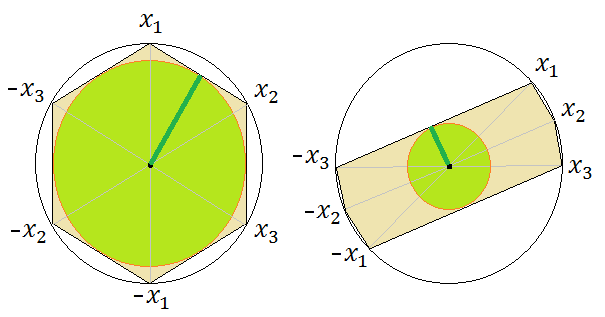
\includegraphics[width=0.7\linewidth]{pics/inradius.png}\\
  \caption{数据点分布和其内接球半径的关系,内接球半径可以度量这些店能否很好地表示子空间。}
  \label{fig:inradius}
\end{figure}

我们有如下引理。

\begin{lemma}\label{lemma:circum_inradius}
  若对于矩阵 $A \in \R^{m \times n}$, 存在 $r>0$,使得
  $$\|Ax\|_2 \leq 1 \quad \forall x \in \cB(0, r),$$
  其中$\cB(0, r)$ 表示 $\R^n$ 中的半径为$r$的欧式球。
  那么$\|A\|_2 \leq \frac{1}{r}$。
\end{lemma}
\begin{proof}
  设$A$ 的svd为$U\Sigma V^T$,取$x=rV_1$,则
  $$\|Ax\|_2 = r \|U \Sigma V^T V_1\|_2 = r \sigma_1 \leq 1.$$
  所以$\|A\|_2 = \sigma_1 \leq \frac{1}{r}$。
\end{proof}

\begin{lemma}\label{lemma:Y_containing_set}
  若矩阵 $X=Y+Z$,令 $\rho:=\max_{i}\|\mathbb{P}_\mathcal{S}z_i\|$, 且 $Y_i \in \mathcal{S}$ 其中
  $\mathcal{S}$ 是线性子空间, 那么我们有:
  \begin{equation*}
    r(\mathrm{Proj}_\mathcal{S} (\mathcal{P}(X))) \geq r(\mathcal{P}(Y)) - \rho
  \end{equation*}
\end{lemma}
\begin{proof}
  首先注意到投影算子是线性算子, 因此 $\mathrm{Proj}_\mathcal{S}(\mathcal{P}(X))=\mathcal{P}(\mathbb{P}_\mathcal{S} X)$。
  根据定义 $\mathcal{P}(\mathbb{P}_\mathcal{S} X)$ 的边界是集合 $\mathcal{B}:=
  \left\{y\text{ }|\text{ }y=\mathbb{P}_\mathcal{S} X c; \|c\|_1=1\right\}$。
  内接球是凸包内的最大球,因此 $r(\mathcal{P}(\mathbb{P}_\mathcal{S} X)) =
  \min_{y\in \mathcal{B}} \|y\|$。 对$y \in \mathcal{B} $ 我们给出下界:
  \begin{align*}
    \|y\| \geq& \|Yc\|-\|\mathbb{P}_\mathcal{S}Z c\|\geq r(\mathcal{P}(Y)) - {\sum}_j{\|\mathbb{P}_\mathcal{S}z_j}\||c_j|
    \geq r(\mathcal{P}(Y)) - \rho\|c\|_1.
  \end{align*}
  因此得证。
\end{proof}

根据\eqref{eq:Geometric_dual},引理~\ref{lemma:circum_inradius} 和引理~\ref{lemma:Y_containing_set},
我们可给出$N_{\parallel}$的上界:
\begin{align}
  \|N_{\parallel}\|_2 \leq& \frac{1+\delta\|N_{\perp}\|}
  {r(\mathcal{P}(Y_{I^c}^{(\ell)}+\mathbb{P}_{\mathcal{S}_{\ell}}(Z_{I^c}^{(\ell)}))}
  \nonumber \\
  =& \frac{1+\delta\|N_{\perp}\|}{r(\mathrm{Proj}_\mathcal{S_{\ell}}
  (\mathcal{P}(X_{I^c}^{(\ell)})))} \nonumber \\
  \leq& \frac{1+\delta\|N_{\perp}\|}{r{\left( \mathcal{Q}_{I^c}^{\ell}\right)}-\delta_1}.\label{eq:nu1_bound}
\end{align}
这个上界依赖于 $\|N_{\perp}\|_2$, 接下来我们将对其进行分析。

\subsubsection{控制$\|N_{\perp}\|_2$}

由于 $N$ 是 $\mathbf{D}_1$ 的最优解,由对偶问题的性质,我们有
$$ N=\lambda E=\lambda(X_I-X^{(\ell)}_{I^c}C). $$
将 $N$ 投影到 $\mathcal{S}^{\perp}_{\ell}$, 我们得到
$N_{\perp}=\lambda \mathbb{P}_{\mathcal{S}_{\ell}^{\perp}}(X_I-X^{(\ell)}_{I^c}C)
= \lambda \mathbb{P}_{\mathcal{S}_{\ell}^{\perp}}(Z_I-Z^{(\ell)}_{I^c}C)^2$.
于是
\begin{align}
  \|N_{\perp}\|_2 & = \max_{\|y\|_2=1} \|N_{\perp}^T y\|_2 \nonumber \\
  & \leq\lambda \left(\|\mathbb{P}_{\mathcal{S}_{\ell}^{\perp}}Z_I\|_2
  +\|C^T (\mathbb{P}_{\mathcal{S}_{\ell}^{\perp}}Z^{(\ell)}_{I^c})^T y\|_2\right)\nonumber\\
  & \leq \lambda\left( \sqrt{m} \delta + \|C^T \ty\|_2\right) \nonumber\\
  & \leq \lambda\left( \sqrt{m} \delta + \sum_j |\ty_j|\|C^T_j\|_2\right) \nonumber\\
  & \leq \lambda\left( \sqrt{m} \delta + \|\ty\|_{\infty}\|C^T\|_{2,1}\right) \nonumber\\
  & \leq \lambda \delta(\Cgl+\sqrt{m}) \leq \lambda\delta\sqrt{m}(\Cgl+1). \label{eq:bounding_nu2}
\end{align}
其中$m$ 为指标集 $I$中的元素个数,$\ty=\mathbb{P}_{\mathcal{S}_{\ell}^{\perp}}Z^{(\ell)}_{I^c})^Ty$,
因此$\|\ty\|_{\infty} \leq \|z_i\|_2 \|y\|_2 \leq \delta$。

下面我们给出 $\Cgl$的上界。
因为 $(C,E)$ 是 \eqref{eq:Opt_fictitious2} 的最优解,所以对任何可行解 $(\tC ,\tE)$
都有 $\Cgl+\frac{\lambda}{2}\|E\|^2_F \leq \tCgl+\frac{\lambda}{2}\|\tilde{E}\|_F^2$。
令 $\tC$ 为下面优化问题的解
\begin{align}\label{eq:Opt_y only}
\min_{c} \; \Cgl \quad
s.t. \quad Y^{(\ell)}_I=Y^{(\ell)}_{I^c}C,
\end{align}
由强对偶性,
$$\tCgl = \max_{N}\left\{\langle N,Y^{(\ell)}_I\rangle | \|N^T
Y^{(\ell)}_{I^c}\|_{2, \infty}\leq 1\right\}.$$
根据引理~\ref{lemma:circum_inradius}, 对偶问题的最优解 $\tilde{N}$ 满足
$\|\tilde{N}\|_2 \leq \frac{1}{r(\mathcal{Q}_{I^c}^{\ell})}$。于是
$$\tCgl = \langle\tilde{N},Y^{(\ell)}_I\rangle \leq \frac{m}{r(\mathcal{Q}_{I^c}^{\ell})}.$$

同时 $\tilde{E} = Z_I - Z_{I^c}^{(\ell)}\tC$, 所以 
$$\|\tilde{E}\|_F^2 \leq (\|Z_I\|+\sum_{j,k} \|z_j\||\tC_{j,k}|)^2
\leq \delta^2 (\sqrt{m} + \|\tC\|_1)^2\leq m \delta^2(1+ \tCgl),$$
于是
$$\Cgl \leq \tCgl + \frac{\lambda}{2}\|\tilde{E}\|_F^2-\frac{\lambda}{2}\|E\|_F^2
\leq \frac{m}{r{(\mathcal{Q}_{I^c}^{\ell})}}+\frac{\lambda}{2}m\delta^2
\left[1+\frac{m}{r{(\mathcal{Q}_{I^c}^{\ell})}}\right]^2-\frac{1}{2\lambda}\|N_{\perp}\|_2^2.$$
注意到 $\frac{\lambda}{2}\|E\|_F^2=\frac{1}{2\lambda}\|N\|_F^2
\geq\frac{1}{2\lambda}\|N_{\perp}\|_F^2 \geq\frac{1}{2\lambda}\|N_{\perp}\|_2^2$。
将 $\tCgl$ 的界带入 \eqref{eq:bounding_nu2} 
\begin{align*}
  &&\;&\|N_{\perp}\|_2 \leq \lambda \delta \sqrt{m} 
  \left(\frac{m}{r(\mathcal{Q}_{I^c}^{\ell})}+\frac{\lambda}{2}\delta^2m
  \left[1+\frac{m}{r(\mathcal{Q}_{I^c}^{\ell})}\right]^2+1\right)
  -\frac{\delta}{2}\sqrt{m}\|N_{\perp}\|_2^2\\
  \Leftrightarrow&&\;
  &\|N_{\perp}\|_2+\frac{\delta}{2}\sqrt{m}\|N_{\perp}\|_2^2\leq
  \lambda\delta\sqrt{m}\left(\frac{m}{r(\mathcal{Q}_{I^c}^{\ell})}+1\right)+
  \frac{\delta}{2}\sqrt{m} \left[\lambda\delta\sqrt{m}
  \left(\frac{m}{r(\mathcal{Q}_{I^c}^{\ell})}+1\right)\right]^2 .
\end{align*}
由于函数 $f(\alpha)=\alpha+\frac{\delta}{2}\sqrt{m}\alpha^2$ 在 $\alpha>0$
时单调递增,则上面的不等式可以推出
\begin{equation}\label{eq:nu2_bound}
  \|N_{\perp}\|_2 \leq \lambda\delta\sqrt{m}\left(\frac{m}{r(\mathcal{Q}_{I^c}^{\ell})}+1\right),
\end{equation}
即我们需要的 $\|N_{\perp}\|_2$ 的上界。

\subsubsection{ $\|N^T x\|_2<1$ 所需的条件}
%\vspace{15pt}
%\noindent{\large \textbf{Conditions for $|\langle x, N \rangle|<1$:} }
结合 \eqref{eq:showing_dual_sep_cond}, \eqref{eq:nu1_bound} 和 \eqref{eq:nu2_bound}, 
我们可以得出 $\|N^T x\|_2$ 的上界:
\begin{align*}
  &\|N^T x\|_2 \leq (\mu(\mathcal{X}_{\ell})+\|\mathbb{P}_{\mathcal{S}_{\ell}}z\|) 
  \|N_{\parallel}\|_2+(\|y\|+\|\mathbb{P}_{\mathcal{S}_{\ell}^{\perp}}z\|)\|N_{\perp}\|_2\\
  \leq&\frac{\mu(\mathcal{X}_{\ell})+\delta_1}{r{\left( \mathcal{Q}_{I^c}^{\ell}\right)}-\delta_1}
  +\left(\frac{(\mu(\mathcal{X}_{\ell})+\delta_1)\delta}{r{\left( \mathcal{Q}_{I^c}^{\ell}\right)}-\delta_1}+1+\delta\right)
  \|N_{\perp}\|_2\\
  \leq& \frac{\mu(\mathcal{X}_{\ell})+\delta_1}{r{\left( \mathcal{Q}_{I^c}^{\ell}\right)}-\delta_1} +
  \lambda\delta(1+\delta)\sqrt{m} \left(\frac{m}{r(\mathcal{Q}_{I^c}^{\ell})}+1\right)
  + \frac{\lambda\delta^2\sqrt{m}(\mu(\mathcal{X}_{\ell})+\delta_1)}
  {r{\left( \mathcal{Q}_{I^c}^{\ell}\right)}-\delta_1}\left(\frac{m}{r(\mathcal{Q}_{I^c}^{\ell})}+1\right).
\end{align*}
简单起见,我们把第二个 $r(\mathcal{Q}_{I^c}^{\ell})$ 松弛成 $r(\mathcal{Q}_{I^c}^{\ell})-\delta_1$。
这样对偶分离条件就被下式保证
\begin{align*}
  \frac{\mu(\mathcal{X}_{\ell})+\delta_1 +\lambda m^{3/2}\delta(1+\delta)+
  \lambda\sqrt{m}\delta^2(\mu(\mathcal{X}_{\ell})+\delta_1)}
  {r{\left( \mathcal{Q}_{I^c}^{\ell}\right)}-\delta_1}
  + \lambda\sqrt{m}\delta(1+\delta)+\frac{\lambda\delta^2 m^{3/2}(\mu(\mathcal{X}_{\ell})+\delta_1)}
  {r{\left( \mathcal{Q}_{I^c}^{\ell}\right)}(r{\left( \mathcal{Q}_{I^c}^{\ell}\right)}-\delta_1)}  < 1.
\end{align*}
记 $\rho:=\lambda\sqrt{m}\delta$, 假设 $\delta<r{\left( \mathcal{Q}_{I^c}^{\ell}\right)}$,
$(\mu(\mathcal{X}_{\ell})+\delta_1)<1$ ,那么我们有下面的不等式
\begin{align*}
  \frac{\lambda\sqrt{m}\delta^2(\mu(\mathcal{X}_{\ell})+\delta_1)}
  {r{\left( \mathcal{Q}_{I^c}^{\ell}\right)}-\delta_1}
  +\frac{\lambda\delta^2 m^{3/2}(\mu(\mathcal{X}_{\ell})+\delta_1)}
  {r{\left( \mathcal{Q}_{I^c}^{\ell}\right)}(r{\left( \mathcal{Q}_{I^c}^{\ell}\right)}-\delta_1)}
  < \frac{\rho (m+\delta)}{r{\left( \mathcal{Q}_{I^c}^{\ell}\right)}-\delta_1}.
\end{align*}
将上式带入化简,我们就得到了一个充分条件
%\begin{equation}\label{eq:dual_cond_simp}
%    \mu < \left(1-\rho\right)r(\mathcal{Q}_{I^c}^{\ell}) +\delta_1\rho-\rho-2\delta_1.
%\end{equation}
\begin{equation}\label{eq:dual_cond_simp}
  \mu(\mathcal{X}_{\ell}) +\rho [2m+(1+m)\delta] +\delta_1
  < \left(1-\rho(1+\delta)\right)(r(\mathcal{Q}_{I^c}^{\ell})-\delta_1).
\end{equation}
把 \eqref{eq:dual_cond_simp} 一般化到所有子空间的所有数据点上,
则必须对每个$\ell = 1,...,k$ 成立:
\begin{equation}\label{eq:Thm1_all}
  \mu(\mathcal{X}_{\ell}) +\rho [2m+(1+m)\delta] +\delta_1
  < \left(1-\rho(1+\delta)\right)\left(\min_{\{I: I\in I(\ell)\}}r(\mathcal{Q}^{(\ell)}_{I^c})-\delta_1\right).
\end{equation}

\subsection{避免平凡解}\label{sec:avoid_trivial}
除了满足 SEP 以外, 我们还要要求问题的解是非平凡的。 不难看出,只要当 $\lambda$
足够大时, 平凡解 $C^* = 0$, $E^*=X_I^{(\ell)}$ 肯定不是最优解。

\begin{lemma}\label{lemma:avoid_trivial}
  对于 \eqref{eq:Opt_A_general} ,当 $\lambda > \frac{1}{\max_{i,j} |X_i^T
Y_j|}$ 时,其最优解一定是非平凡的。
\end{lemma}

\begin{proof}
  我们只要说明存在一个非平凡解比平凡解更优即可。 设 $i, j$ 为 $|X_i^T
  Y_j|$ 取到最大时的下标, 取 $C_{i,j} = a$ 其余取为$0$, 则$C$
  非平凡。我们有
  $$ \frac{\lambda}{2} \|Y_j - X_i a \|_2^2 + |a| = \frac{\lambda}{2}
  \|Y_j\|_2^2 + \frac{\lambda}{2} \|X_i\|_2^2 a^2 +\left( 1-\lambda |X_i^T Y_j|
  \right)a, $$
  其中取 $a = \frac{\lambda |X_i^T Y_j|-1}{\lambda \|X_i\|_2^2} \sign(X_i^T Y_j)$
  则上式成立且等于
  $$ \frac{\lambda}{2} \|Y_j\|_2^2 - \frac{(\lambda|X_i^T Y_j| -1)^2}
  {2 \lambda \|X_i\|_2^2 } < \frac{\lambda}{2} \|Y_j\|_2^2. $$
  因此最优解一定非平凡。
\end{proof}

在对偶分离的条件下,我们只需要考虑在同一个子空间下的点。因此 $\|X_{I^c}^T X_I\|_{\infty} = 
\left\|[X_{I^c}^{(\ell)}]^T X_I\right\|_{\infty}$. 令 $i_0, j_0$ 为矩阵
$[X_{I^c}^{(\ell)}]^T X_I$ 取到最大绝对值的位置, $i,j$ 为矩阵
$[Y_{I^c}^{(\ell)}]^T Y_i$ 取到最大绝对值的位置(如果有不止一个就任选一个),
我们有
\begin{align}
  \left\|[X_{I^c}^{(\ell)}]^TX_I\right\|_{\infty}&=\left|\langle x_{i_0},
  x_{j_0}\rangle\right|  \geq \left|\langle x_i, x_j\rangle\right|\nonumber\\
  &= \left|\langle y_i, y_j\rangle  + \langle y_i, z_j\rangle + \langle z_i, y_j\rangle + \langle z_i, z_j\rangle\right|\nonumber\\
  &\geq \left|\langle y_i, y_j\rangle\right| - \left|\langle y_i, z_j\rangle + \langle z_i, y_j\rangle + \langle z_i, z_j\rangle\right|\nonumber\\
  & = \left\|[Y_{I^c}^{(\ell)}]^Ty_i\right\|_{\infty} - \left|\langle y_i, z_j\rangle + \langle z_i, y_j\rangle + \langle z_i, z_j\rangle\right|\nonumber\\
  &\geq r(\mathcal{Q}^{(\ell)}_{I^c}) - 2\delta - \delta^2. \label{eq:lowerbounding_max_affinity}
\end{align}
其中 $x_i, x_{i_0}$ 表示 $X_{I^c}^{\ell}$ 矩阵的第 $i$ 和 $i_0$ 列,$x_j,
x_{j_0}$ 表示 $X_I^{\ell}$ 的第 $j$ 和 $j_0$ 列, $y_i$ 是 $Y_{I^c}^{\ell}$
的第 $i$ 列, $y_j$ 是 $Y_I^{\ell}$ 的第 $j$ 列。 最后一个不等式成立是因为 $\mathcal{Q}^{(\ell)}_{I^c}$ 
的内接球半径是集合 $\left\{\left\| [ Y_{I^c}^{(\ell)}]^T w\right\|_\infty: w
\in  \mathcal{S}_{\ell}\right\} $ 的下界。因此只要
\begin{equation}\label{eq:lambda_low}
  \lambda > \frac{1}{ r(\mathcal{Q}^{(\ell)}_{I^c}) - 2\delta - \delta^2},
\end{equation}
\eqref{eq:Opt_fictitious2}的解就是非平凡的。

%\subsection{存在适当的$\lambda$}\label{sec:exist_lambda}
%
%对于所有 $\ell=1,...,L$,\eqref{eq:Thm1_all} 和 \eqref{eq:lambda_low}
%必须被同时满足。 \eqref{eq:lambda_low} 给出了 $\lambda$ 的下界而 \eqref{eq:Thm1_all}
%给出了上界。 重复下上面的记号 $r_{\ell}:=\min_{\{i: x_i\in X^{(\ell)}\}}r(\mathcal{Q}^{(\ell)}_{I^c})$,
%$\mu_{\ell}:=\mu(\mathcal{X}_{\ell})$ and $r=\min_{\ell} r_{\ell}$, the condition on $\lambda$ is:
%%Denote $r_{\ell}:=\min_{\{i: x_i\in X^{(\ell)}\}}r(\mathcal{Q}^{(\ell)}_{I^c})$, $\mu_{\ell}:=\mu(\mathcal{X}_{\ell})$, the condition on $\lambda$ is:
%\begin{align*}
%  \max_{\ell}\frac{1}{r_{\ell} - 2\delta-\delta^2}<\lambda < \min_{\ell}\frac{r_{\ell}-\mu_{\ell}-2\delta_1}{\delta(1+\delta)(2+r_{\ell}-\delta_1)}.
%\end{align*}
%%Note that on the left
%With the observation that
%\begin{align*}
%\max_{\ell}\frac{1}{r_{\ell} - 2\delta-\delta^2}
%= \frac{1}{\min r_{\ell} - 2\delta-\delta^2},
%\end{align*}
%% On the right
%% $$\min_{\ell}\left\{\frac{r_{\ell}-\mu_{\ell}-2\delta_1}{\delta(1+\delta)(3+2r_{\ell}-2\delta_1)}\right\} = \frac{\min_{\ell}r_{\ell}-\mu_{\ell}-2\delta_1}{\delta(1+\delta)(3+2\min_{\ell}r_{\ell}-2\delta_1)}.$$
%%Denote $r=\min_{\ell} r_{\ell}$,
%it suffices to require $\lambda$ to obey for each $\ell$:
%\begin{equation}\label{eq:lambda_range}
%\frac{1}{r - 2\delta-\delta^2}<
%        \lambda<\frac{r_{\ell}-\mu_{\ell}-2\delta_1}{\delta(1+\delta)(2+r_{\ell}-\delta_1)}.
%\end{equation}
%
%
%
%%To understand this, when $\delta$ and $\mu$ is small then any $\lambda$ values satisfying $\Theta(1/r)<\lambda<\Theta(r/\delta)$ will satisfy separation condition.
%
%%We will now derive the condition on $\delta$ such that \eqref{eq:lambda_range} is not an empty set.
%
%
%We will now show that under condition \eqref{eq:deterministic_delta}, the range \eqref{eq:lambda_range} is not an empty set. Again, we relax $\delta_1$ to $\delta$ in \eqref{eq:lambda_range} and get
%\begin{equation}\label{eq:nonempty_cond}
%  \frac{1}{r - 2\delta-\delta^2}< \frac{r_{\ell}-\mu_{\ell}-2\delta}{\delta(1+\delta)(2+r_{\ell}-\delta)}.
%\end{equation}
%Since all denominators are positive, we obtain the standard form of the inequality
%$$ A\delta^3+B\delta^2+C\delta+D<0 $$ with
%$$
%\begin{cases}
%A=-3\leq 0\\
%B=-3+2(r_\ell-\mu_\ell) + r_\ell \leq 0\\%-(6r-r_{\ell}+7-\mu_{\ell})\\
%C=2+4(r_{\ell}-\mu_{\ell})+r_\ell+2r \leq 2+7r_{\ell}\\%2+r_{\ell}+2r+(r_{\ell}-\mu_{\ell})(2r+3)\\%3r_{\ell}r+6r_{\ell}+2r-3\mu_{\ell} r+3-4\mu_{\ell}\\
%D=-r(r_{\ell}-\mu_{\ell})
%\end{cases}
%$$
%Check that \eqref{eq:deterministic_delta} is sufficient for the above $3$rd order inequality to hold. Therefore,
%$$\eqref{eq:deterministic_delta}\Rightarrow A\delta^3+B\delta^2+C\delta+D<0 \Leftrightarrow \eqref{eq:nonempty_cond}
%\Rightarrow \text{\eqref{eq:lambda_range} is not an empty set.}$$
%%This completes the proof of Theorem~\ref{thm:thm_general}.
%
\end{document}
